% Chapter 4

\chapter{Methodology} % Write in your own chapter title
\label{Chapter4}
\lhead{Chapter 4. \emph{Methodology}} % Write in your own chapter title to set the page header
In this chapter the real game dataset and the implementation of MapReduce k-means clustering algorithm is described. There is a section about preprocessing the data, constructing the player behaviour features and explaining the MR k-means implementation process and the MR k-means program that launches the MR algorithm in each iteration, incrementally clustering multiple batches of data. 

In GA the user telemetry data arrives in mini batches from the games, a batch each day. In this thesis the idea is then to process each batch and incrementally cluster the data, where the output from one batch is the input to the next.

An incremental MR k-means clustering algorithm and apply it on multiple batches of the game metric data to find average player behaviour described by a the constructed player behavioural feature vector. The algorithm is highly scalable and can easily be executed on numerous virtual computers using the Amazon Elastic MapReduce (Amazon EMR) web service. 

Different MR k-means implementation were tried in the process of this thesis and different efficient computation methods were compared on a larger generated dataset, including scalability (scale-up and scale-out) tests running on different cluster setups in the Amazon EMR. In the last section a quick overview of the development environment and tools that were used in this thesis is covered.

\section{Dataset}
\label{sec:realdataset}
The dataset is from a Free-to-Play (F2P) online game that is available on Google Plus and Facebook. This real life game dataset is from one of the many games that GameAnalytics is analyzing for their customers. Because of a confidentiality agreement its name is not mentioned in this thesis, but lets call it \textit{Free Battle Online}. Same is about the real names of events or features in the dataset is fictional, this unfortunately means that there is a very limited knowledge about the data, e.g. what individual events mean and the timespan. The goal of the game is to fight battles against both non-playing-characters (NPCs) and other players. You can click on various places to travel to finish battle missions or just visit other players and initiate battles to steal their resources.

The dataset is a user telemetry data, e.g. user behavioural events, where each line represents an action performed by the user or is a direct influence from a user behaviour. There are over $5.100.000$ rows in this data set, with approx. $550$ unique events generated by approx. $94.000$ players. Average events per player is $\mu = 54$ with standard deviation $\sigma = 145$, indicating that the data is spread out over a wide range of values. The measure of the spread is in Table~\ref{tab:FiveSummaryEvents} showing the five number summary; The first quartile $Q_1$ cuts off the lowest $25\%$ of the data, the second quartile gives the center of the distributions known as the $Median$, the third quartile $Q_3$ cuts of the highest $25\%$. The median is lower than the mean of the data describing a positively skewed distribution, see Figure~\ref{fig:boxplot_events} for a visualization of the distribution.

\begin{table}[h]
\centering
\begin{tabular}{| l | r | r | r | r | r |}
    \hline
    & \textit{Min} & $Q_1$ & \textit{Median} & $Q_3$ & \textit{Max} \\ \hline
    Events & 1 & 4 & 23 & 61 & 10865 \\ \hline
\end{tabular}
\caption{This table shows the five number summary about the number of events generated by each unique player in the dataset.}
\label{tab:FiveSummaryEvents}
\end{table}


\begin{figure}[here]
\centerline{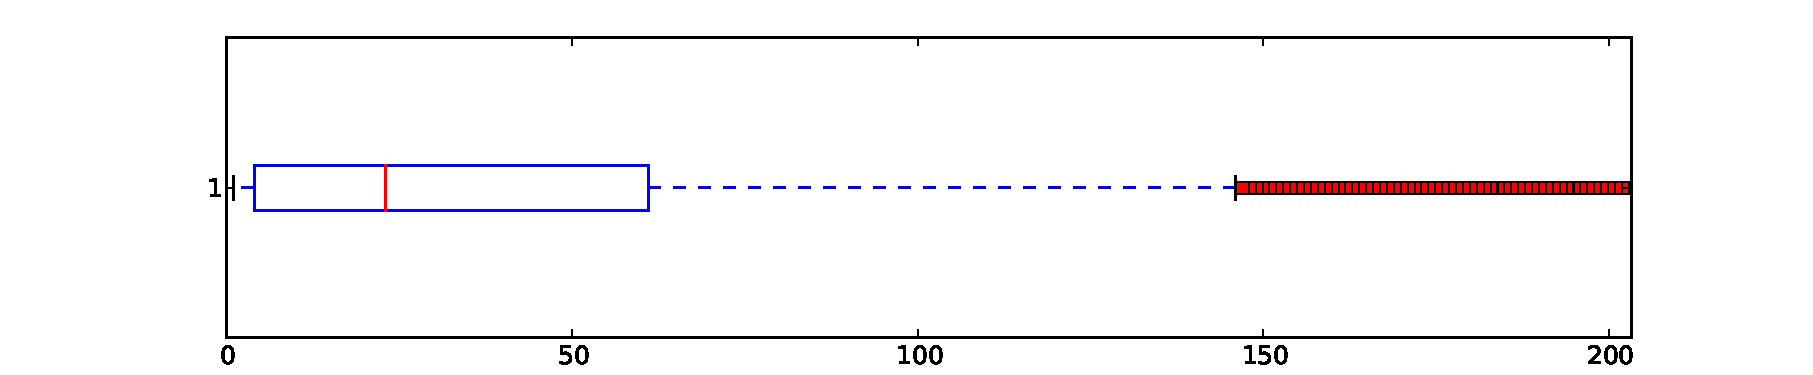
\includegraphics[width=0.9\textwidth]{Figures/boxplot_events.pdf}}
\caption{A boxplot visualizing the Events distribution incorporating the five number summary.}
\label{fig:boxplot_events}
\end{figure}

The two lines outside the box in Figure~\ref{fig:boxplot_events} are called whiskers and represent the extreme low and high values that are less than $1.5 \times IQR$ beyond the quartiles, IQR is an interquartile range defined as $Q3 - Q1$ a range covered by the middle half of the data. The first and third quartiles represent the ends of the box and the median is the red line. The red \textit{squares} are individual points called \textit{outliers}. Only about $6\%$ or $\approx 5500$ players of the entire population generated more than 150 events, $0.3\%$ or $\approx300$ players have more than 1000 events and less than ten people have a range of $5.000-10.000$ generated events! A histogram showing the frequency of events generated by players is shown in Figure~\ref{fig:histogram_events_iqr}, zooming in on the spread that gives the range covered by the middle half of the data.

\begin{figure}[here]
\centerline{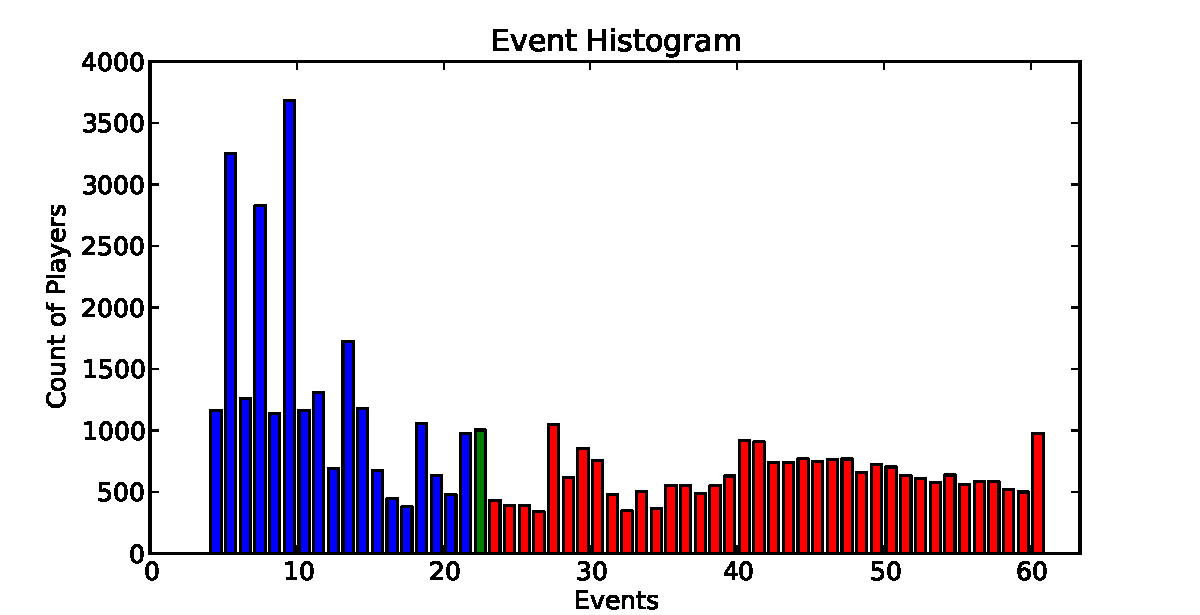
\includegraphics[width=0.9\textwidth]{Figures/histogram_events_iqr.pdf}}
\caption{A histogram for number of events using singleton buckets in the interquartile range, defined as $Q3 - Q1$, range covered by the middle half of the data.}
\label{fig:histogram_events_iqr}
\end{figure}


\subsection{Game Metric Construction}
\label{gamemetric}
For this thesis the number of game features were kept at minimal and it was decided to build the feature vector with three features. Given the limited knowledge and information that were available about individual events, it was decided to select events that had high frequency compared to other events and hopefully could describe different behaviour between groups of players in those features. A $3-dimensional$ feature vector was constructed for each unique player, containing a frequency of three events generated by the player. The aggregated events are:
\begin{itemize}
\item Login: Number of logins/access into different areas in the game($\mu = 2.4, \sigma = 4.8$)
\item Battle: Number of battles this player have started ($\mu = 3.7, \sigma = 9.6$)
\item Premium Spending: Number of times this player spends a in-game money on virtual items or resources ($\mu = 1.1, \sigma = 2.7$) 
\end{itemize}

Features were chosen such that they could describe player engagement to the game. How active the player is exploring various areas, fighting battles and spending in-game money to advance in the game quicker, see Figure~\ref{fig:DatasetZdata} how the data looks like in data space. 

The five number summary of the skewed distribution is in Table~\ref{tab:FiveSummaryLoginsBattlesPremium}. Boxplots visualizing the distributions for these events are shown in relevant figures below; Logins in Figure~\ref{fig:boxplot_logins}, Battles in Figure~\ref{fig:boxplot_battles} and Premium spent events in Figure~\ref{fig:boxplot_premium}.

\begin{figure}[here]
\centerline{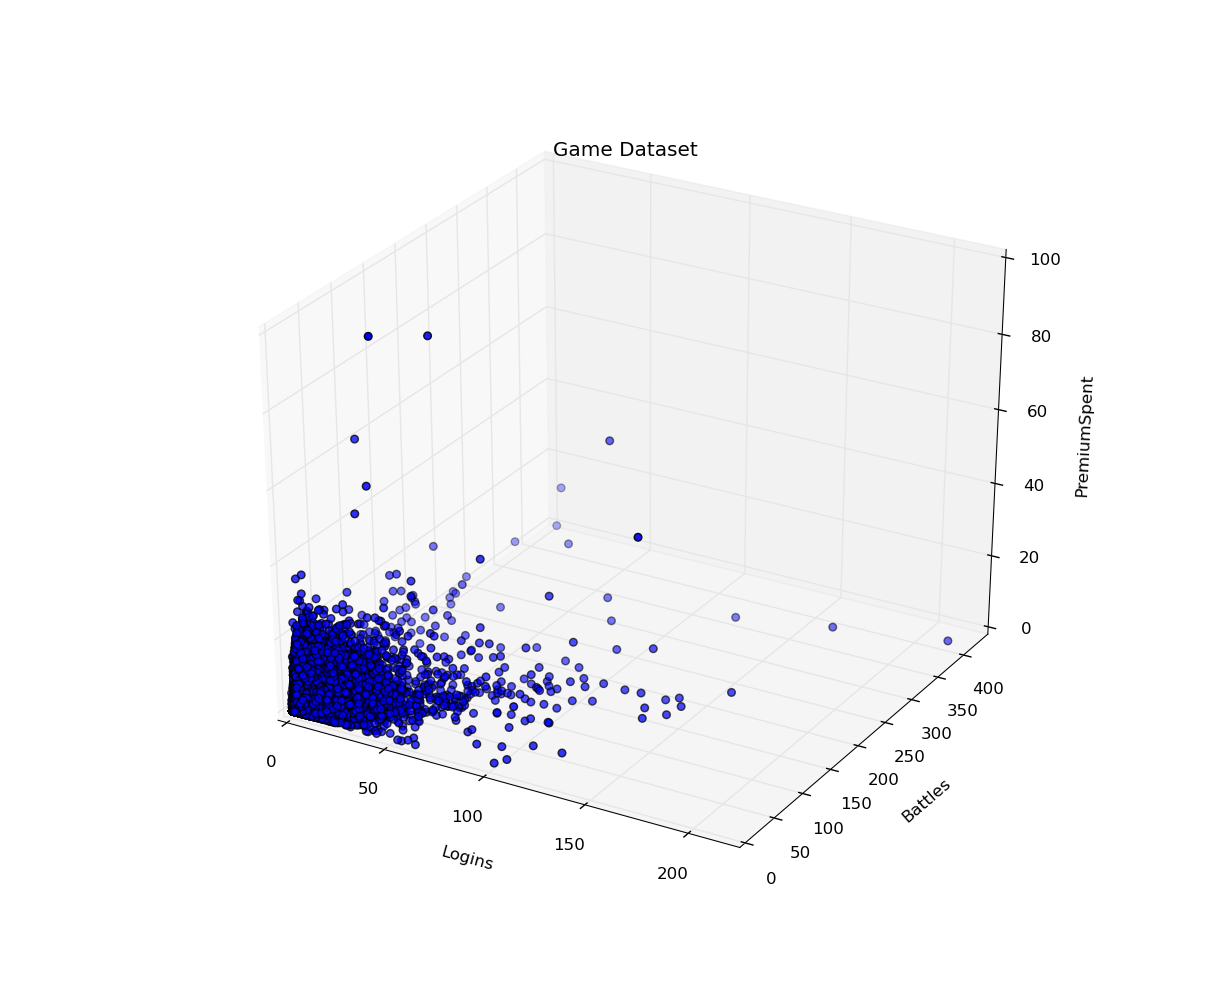
\includegraphics[trim = 10mm 20mm 10mm 30mm, clip, width=0.9\textwidth]{Figures/DatasetZdataWholerealgamedataset.png}}
\caption{This figure shows the whole game metric dataset plotted in $3$-dimensional data space. Showing the whole range for the data features.}
\label{fig:DatasetZdata}
\end{figure}


\begin{table}[h]
\centering
\begin{tabular}{| l | r | r | r | r | r |}
    \hline
    & \textit{Min} & $Q_1$ & \textit{Median} & $Q_3$ & \textit{Max} \\ \hline
    Logins & 0 & 1 & 1 & 2 & 220 \\ \hline
    Battles & 0 & 0 & 1 & 4 & 439 \\ \hline
    Premium spent & 0 & 0 & 0 & 1 & 100 \\ \hline
\end{tabular}
\caption{This table shows the five number summary for the Logins, Battles and Premium spent events generated by each unique player in the dataset.}
\label{tab:FiveSummaryLoginsBattlesPremium}
\end{table}



The features values are spread out over large range of values, in the preprocessing Section~\ref{preprocessing} it is explained how the outliers or anomalies were detected and removed from the data before applying the MR k-means algorithm using a \textit{z-score} method.

\begin{center}
\begin{figure}[h]
\centerline{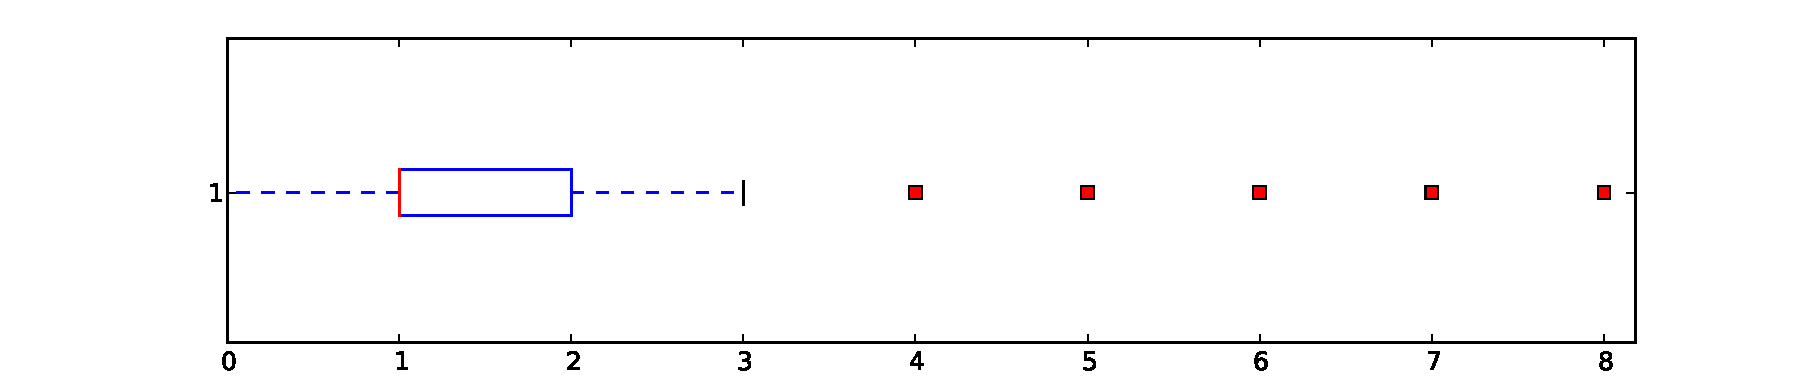
\includegraphics[width=0.9\textwidth]{Figures/boxplot_logins.pdf}}
\caption{A boxplot visualizing the Login events distribution incorporating the five number summary.}
\label{fig:boxplot_logins}
\end{figure}

\begin{figure}[h]
\centerline{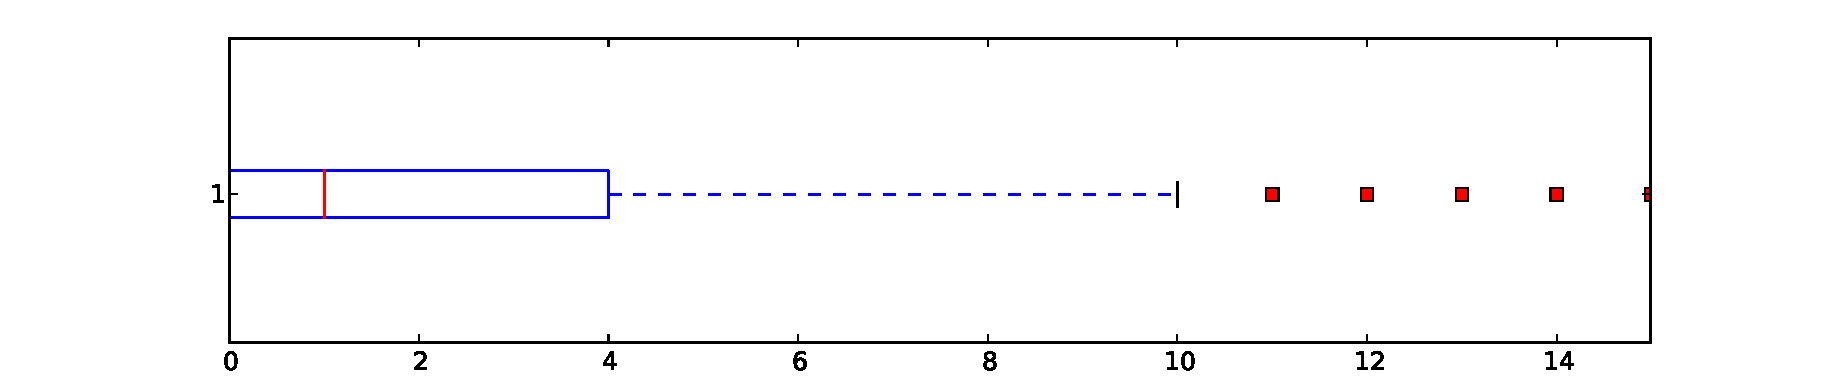
\includegraphics[width=0.9\textwidth]{Figures/boxplot_battles.pdf}}
\caption{A boxplot visualizing the Battle events distribution incorporating the five number summary.}
\label{fig:boxplot_battles}
\end{figure}

\begin{figure}[here]
\centerline{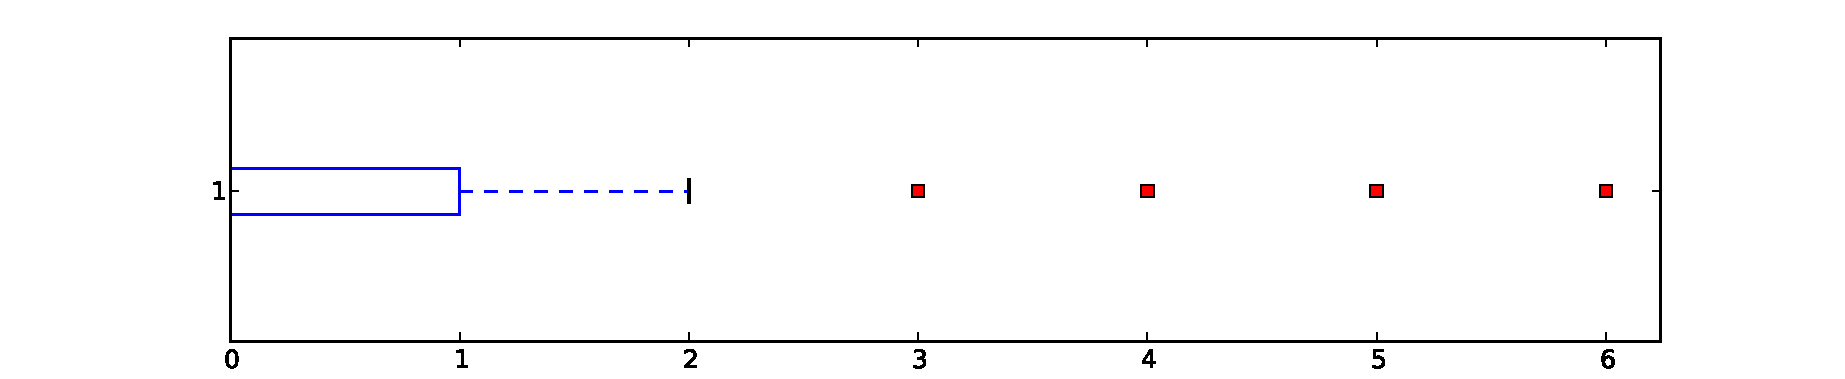
\includegraphics[width=0.9\textwidth]{Figures/boxplot_premiumspent.pdf}}
\caption{A boxplot visualizing the Premium spent events distribution incorporating the five number summary.}
\label{fig:boxplot_premium}
\end{figure}
\end{center}


\subsection{Preprocessing}
\label{preprocessing}
User telemetry from games can be very noisy in that sense it can contain lots of irrelevant events and logging information and even developers from the game studio can generate events. For this dataset the following preprocessing steps were performed:
\begin{itemize}
\item Sort the events after event timestamp.
\item Split the dataset into $10$ approx. equally sized data set pieces.
\item Filter out irrelevant events and logging information. E.g. Events not origin from Facebook or Google Plus, non related events and in game studio debugging generated events.
\item For each data set piece:
 \begin{itemize}
 \item Counting the events mentioned above per user to build the feature vector.
 \item Remove outliers or anomalies from the data.
 \item Standardize the data to standard scores also called \textit{z-score}. Transforming the data
to standard normal distribution, with $\mu = 0$ and $\sigma = 1$. 
 \end{itemize}
\end{itemize}

To apply the incremental MR k-means algorithm it was needed to have multiple batches of data to process incrementally. The real game dataset from GA was used and split up into $10$ equally sized data batches sorted after the event arrival timestamp. The idea was to try to simulate that the algorithm is processing multiple batches of data in the same timely order as the events were generated over multiple time-periods or days, like at GA. Next irrelevant information are filtered out, e.g. information that don't contribute as a event logging or are obviously from the game designers themselves.

Each data batch is processed by aggregating or counting the events that were selected before to build the feature vector for each unique player in the data set. Next the outliers were found by transforming the data to standard scores using the \textit{zero mean normalization} (ZMN), also called \textit{z-score}, with standard normal distribution having zero mean and unit variance $\mu = 0$ and $\sigma = 1$. A feature vector that has a feature value z-score that is more than $3$ standard deviations away from the mean is considered an outlier in the data and is removed from the original data batch. Having a data batch without outliers, the data can be transformed again using ZMN, without having the effect from the outliers. The ZMN is defined as follows


\begin{center}
$z = \dfrac{x  - \mu}{\sigma}$ 
\end{center}


Using ZMN is widely used in machine learning algorithms and is needed when calculating the distance between two points (feature vectors) such that each feature contributes approximately equally to the final distance, see Figure~\ref{fig:DatasetZdataWithoutOutliers}.

\begin{figure}[here]
\centerline{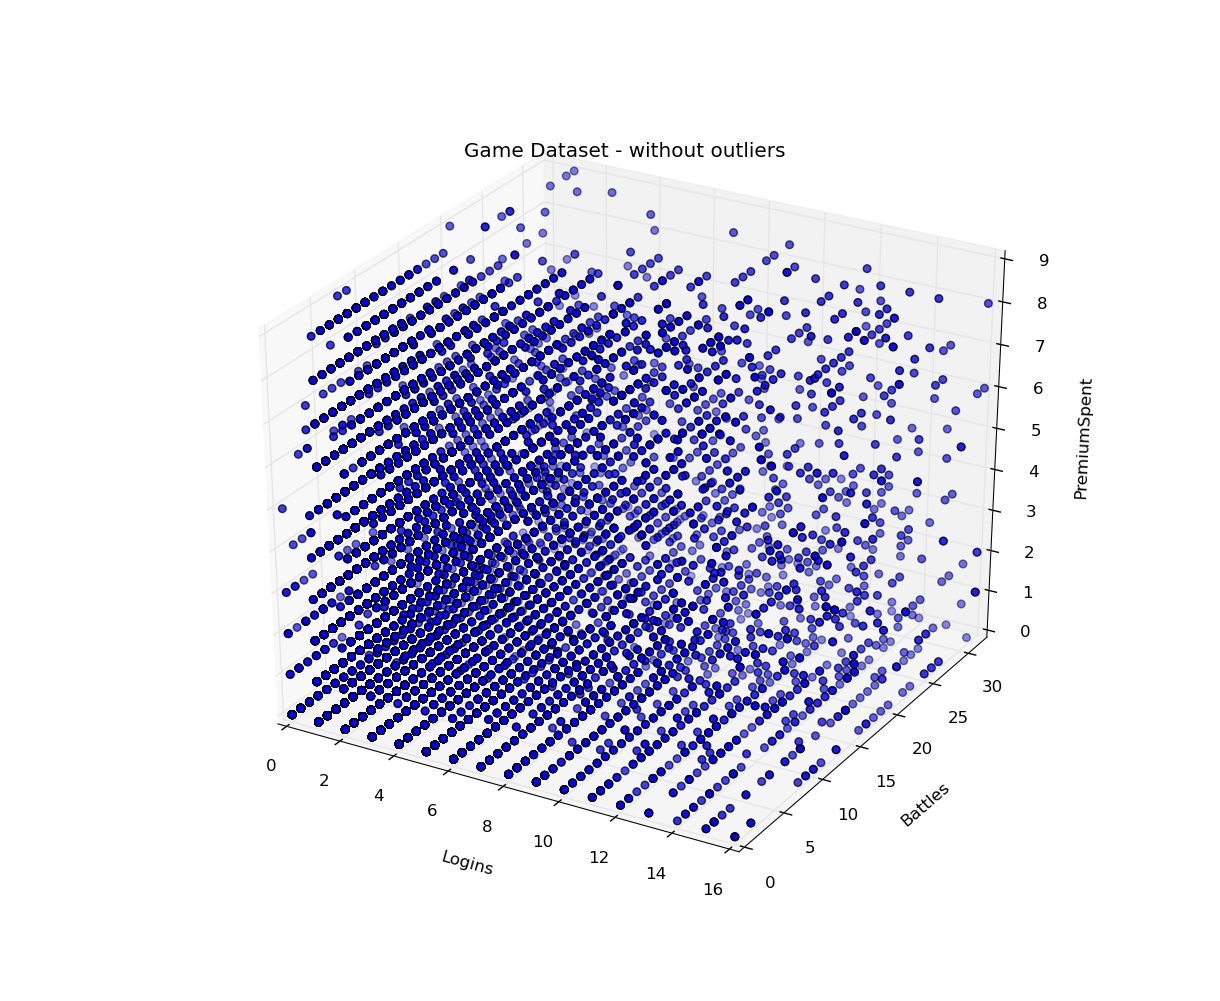
\includegraphics[trim = 10mm 20mm 10mm 30mm, clip, width=0.9\textwidth]{Figures/DatasetZdataWithoutOutliers.png}}
\caption{This figures shows the whole game metric dataset plotted in $3$-dimensional data space, after applying the zscore transformation.}
\label{fig:DatasetZdataWithoutOutliers}
\end{figure}

Removing the outliers from the whole dataset, using the ZMN method described above, the total number of unique players become approx $90.800$ instead of approx. $94.000$, removing $\approx 4\%$ of the population. The five number summary for the whole dataset can be found in Table~\ref{tab:FiveSummaryLoginsBattlesPremiumWoOutliers}, notice the range of values compared to the Table~\ref{tab:FiveSummaryLoginsBattlesPremium} in Section~\ref{gamemetric}. The multiple data batches that get feeded into the clustering algorithm had $\approx 5\%$ player feature vectors removed on average, see Table~\ref{tab:DatabatchesWoOutliers} below.

\begin{table}[h]
\centering
\begin{tabular}{| l | r | r | r | r | r |}
    \hline
    & \textit{Min} & $Q_1$ & \textit{Median} & $Q_3$ & \textit{Max} \\ \hline
    Logins & 2 & 1 & 1 & 2 & 16 \\ \hline
    Battles & 0 & 0 & 1 & 4 & 32 \\ \hline
    Premium spent & 0 & 0 & 0 & 0 & 9 \\ \hline
\end{tabular}
\caption{This table shows the five number summary for the Logins, Battles and Premium spent events generated by each player from the whole dataset with outliers removed.}
\label{tab:FiveSummaryLoginsBattlesPremiumWoOutliers}
\end{table}


\begin{table}[h]
\centering
\scalebox{0.8}{%
\begin{tabular}{| l | r | r | r | r | r | r | r | r | r | r |}
    \hline
    & Data 1 & Data 2 & Data 3 & Data 4 & Data 5 & Data 6 & Data 7 & Data 8 & Data 9 & Data 10 \\ \hline
    Players & 14054 & 13365 & 13403 & 13503 & 13441 & 13276 & 12839 & 13413 & 13473 & 13412 \\ \hline
    Outliers  & 658 & 741 & 661 & 673 & 748 & 698 & 685 & 724 & 669 & 680 \\ \hline
    $\%$ removed & $4,68\%$ & $5,44\%$ & $4,93\%$ & $4,98\%$ & $5,56\%$ & $5,25\%$ & $5,33\%$ & $5,39\%$ & $4,96\%$ & $5,07\%$ \\ \hline
\end{tabular}}
\caption{This table shows the player population, number of outliers found and the percentage of the population removed, for each data batch.}
\label{tab:DatabatchesWoOutliers}
\end{table}


\newpage
\section{MapReduce K-means algorithm}
A k-means algorithm was implemented in MapReduce (MR) that is able to incrementally process large-scale datasets in parallel when running on e.g. Amazon EMR. Three versions of MR k-means was implemented, two of them use different MR execution flows, but the final version builds on the second one and introduces a more efficient way of computing the nearest centroid in the Mapper phase. First version was the the naive one that introduces only a \textit{Map} and \textit{Reduce} phase, that assigns each point (feature vector) to a nearest cluster in the Map phase and updates the centroids for the clusters in the Reduce phase. The programmer only needs to fill in two functions, the Mapper and Reducer. 

The other two versions have a \textit{Combiner} phase implemented that performs reduce work on the same computer node as the Mapper, by calculating intermediate sums of all the points for each cluster from a Mapper function. This minimizes the data needed to be transferred and shuffled by the MR framework to the Reducer, sending only an intermediate sum with each centroid from each mapper instead of list of all data points belonging to each cluster.

In the next subsections the three implementations and their pseudo codes are presented. Next will the \textit{MR K-means Program} be explained, that controls the incremental data batch processing by executing $n$ iterations of the MR K-means job. The most computation work in k-means is to find the nearest centroid for a given feature vector by calculating the distance between the two. Three different implementations were done for the nearest centroid function used by the Mapper.

\subsection{MR K-means First Version - Map and Reduce}
\label{sec:kmeansmapreduce}
Implementing the Mapper and a Reducer function version is the most common implementation of k-means in MR, where the Mapper function calculates the nearest centroids to each data point and emits (sends) that pair to the Reducer function that sums up all data point values for each centroid, and outputs updated centroids. The Mapper function is called for each player feature vector found in the data batch, and iterates through all centroids that are stored in memory to calculate the distance to the nearest one. The nearest centroid and its data feature vector are sent from all the Map tasks(in parallel) to the MR framework that shuffles and sorts all feature vectors together which belongs to the same centroid. The pseudo-code for the Mapper function can be found in Algorithm~\ref{alg:mapkmeansv1} and for Reducer in Algorithm~\ref{alg:reducekmeansv1}.

\algsetup{indent=2em}
\begin{center}
\newcommand{\map}{\ensuremath{\mbox{\sc K-means First Version: Mapper}}}
\begin{algorithm}[h!]
\caption{$\map(key,value)$}\label{alg:mapkmeansv1}
\begin{algorithmic}[1]
\REQUIRE $key = document\_name$, $value = feature\_vector$
\ENSURE $key = centroid\_id$, $value = feature\_vector$.
\STATE $current\_centroids \leftarrow C = \{c_1...c_k\}$ \COMMENT{loaded from memory}
\STATE $feature\_vector \leftarrow = value$
\medskip
\STATE $nearestCentroid = getNearestCentroid(feature\_vector, current\_centroids)$
\medskip
\STATE{$EmitIntermediate(nearestCentroid, feature\_vector)$}
\end{algorithmic}
\end{algorithm}
\end{center}



The Reducer function then gets called for each centroid with all of its feature vectors (assigned in the Mapper phase), iterates through all the feature vectors, sums up their values and divides with their count to get a new updated centroid and outputs that centroid, or the mean that represents the average feature vector for the cluster population.

\begin{center}
\newcommand{\map}{\ensuremath{\mbox{\sc K-means First Version: Reducer}}}
\begin{algorithm}[h!]
\caption{$\map(key,values)$}\label{alg:reducekmeansv1}
\begin{algorithmic}[1]
\REQUIRE $key = centroid\_id$, $values = feature\_vector\_list$
\ENSURE $key = centroid\_id$, $value = average\_feature\_vector$.
\STATE $feature\_vector\_list \leftarrow values$
\medskip
\STATE $sum\_feature\_vector \leftarrow [0, 0, 0]$
\FORALL{$feature\_vector \in  feature\_vector\_list$} 
	\STATE $sum\_feature\_vector \leftarrow sum\_feature\_vector + feature\_vector$
\ENDFOR
\medskip
\STATE $count\_feature\_vectors \leftarrow getCount(feature\_vector\_list)$
\STATE $average\_feature\_vector \leftarrow sum\_feature\_vector \div count\_feature\_vectors$
\medskip
\STATE{$Emit(key, average\_feature\_vector)$}
\end{algorithmic}
\end{algorithm}
\end{center}

Finding the nearest centroid to a point by computing the distances to all the $k$ centroids is where the most of the work is done, and is be found in the Mapper phase. See Algorithm~\ref{alg:nearestcentroidnaive} to see the pseudo-code for the \textit{getNearestCentroid()} function.

\begin{center}
\newcommand{\map}{\ensuremath{\mbox{\sc getNearestCentroid}}}
\begin{algorithm}[h!]
\caption{$\map(point, centroids)$}\label{alg:nearestcentroidnaive}
\begin{algorithmic}[1]
\REQUIRE $point = 1 \times d$ \textit{feature array}, $centroids = k \times d$ \textit{array}).
\ENSURE $nearestCentroid = nearest\_centroid\_id$.
\medskip
\STATE $minDistance \leftarrow +\infty$
\STATE $nearestCentroid \leftarrow None$
\FORALL{$centroid$ $c \in centroids$} 
	\STATE $distance = 0$
	\FOR{$feature$ $i$ \TO $d$} 
		\STATE $distance \leftarrow distance + (point[i] - c[i])^2$ \COMMENT {sums up error for each feature}
	\ENDFOR
	\STATE $distance \leftarrow square\_root(distance)$
	\IF{$distance < minDistance$} 
		\STATE $minDistance \leftarrow distance$
		\STATE $nearestCentroid \leftarrow c$
	\ENDIF
\ENDFOR
\medskip
\RETURN {$nearestCentroid$}
\end{algorithmic}
\end{algorithm}
\end{center}


\subsection{MR K-means Second Version - Map, Combiner and Reduce}
\label{sec:MapCombineReduceVersion}
By adding the Combiner phase in between the Map and Reduce phase, one can reduce a large amount of overhead in data transfer and computation in the MapReduce framework. The Combiner phase is executed on the same computer as the Map phase and is thought of as a reduce phase inside the Map phase. The Combiner function takes input directly from the Mapper function and calculates intermediate results that is emitted over the network instead of the Mapper emitting a key and value pair for each feature vector, which can be problematic for large datasets.

\begin{center}
\newcommand{\map}{\ensuremath{\mbox{\sc K-means Second Version: Combiner}}}
\begin{algorithm}[h!]
\caption{$\map(key,values)$}\label{alg:combinekmeansv2}
\begin{algorithmic}[1]
\REQUIRE $key = centroid\_id$, $values = feature\_vector\_list$
\ENSURE $key = centroid\_id$, $value = [sum\_feature\_vector$, $count\_feature\_vectors])$.
\STATE $feature\_vector\_list \leftarrow values$
\medskip
\STATE $sum\_feature\_vector \leftarrow [0, 0, 0]$
\FORALL{$feature\_vector \in  feature\_vector\_list$} 
	\STATE $sum\_feature\_vector \leftarrow sum\_feature\_vector + feature\_vector$
\ENDFOR
\medskip
\STATE $count\_feature\_vectors \leftarrow getCount(feature\_vector\_list)$
\medskip
\STATE{$EmitIntermediate(key, [sum\_feature\_vector$, $count\_feature\_vectors])$}
\end{algorithmic}
\end{algorithm}
\end{center}

In this version the same Mapper function as described above in Algorithm~\ref{alg:mapkmeansv1} is used but the Reducer needs to be changed. The Combiner function however, becomes very similar to the old Reducer in Algorithm~\ref{alg:reducekmeansv1}. The only difference is that the Combiner doesn't compute the average feature vector or the mean, and emits a little more complex key and value pair, where $key = centroid\_id$ and $value = [sum\_feature\_vector$,~$count\_feature\_vectors]$, see pseudo-code in Algorithm~\ref{alg:combinekmeansv2}. 

\begin{center}
\newcommand{\map}{\ensuremath{\mbox{\sc K-means Second Version: Reducer}}}
\begin{algorithm}[h!]
\caption{$\map(key,values)$}\label{alg:reducekmeansv2}
\begin{algorithmic}[1]
\REQUIRE $key = centroid\_id$, $values = [sum\_feature\_vector$, $count\_feature\_vectors])$
\ENSURE $key = centroid\_id$, $value = average\_feature\_vector$.
\STATE $sum\_and\_count\_list \leftarrow values$
\medskip
\STATE $sum\_total\_feature\_vector \leftarrow [0, 0, 0]$
\STATE $count\_total \leftarrow 0$
\FORALL{$sum\_and\_count \in  sum\_and\_count\_list$} 
	\STATE $sum\_vector \leftarrow getSumVector(sum\_and\_count)$
	\STATE $count \leftarrow getCount(sum\_and\_count)$
	\STATE $sum\_total\_feature\_vector \leftarrow sum\_total\_feature\_vector + sum\_vector$
	\STATE $count\_total \leftarrow count\_total + count$
\ENDFOR
\medskip
\STATE $average\_feature\_vector \leftarrow sum\_total\_feature\_vector \div count\_total$
\medskip
\STATE{$Emit(key$, $average\_feature\_vector)$}
\end{algorithmic}
\end{algorithm}
\end{center}

The new Reducer algorithm then sums up the intermediate sums and counts from the Combiners and calculates the average feature vector. The Reducer works with much smaller data as it receives a sum of values per centroid instead of all the feature vectors for each centroid, this is of great help when working with large data and has a much less communication overhead in the MR framework, the pseudo-code for the the Reducer is in Algorithm~\ref{alg:reducekmeansv2}.


\subsection{MR K-means Final Implementation}
\label{sec:kmeansfinalversion}
The final MR k-means implementation builds on the second version in Section~\ref{sec:MapCombineReduceVersion} and differs only in computing the nearest centroid in the Mapper phase. calculating the nearest centroid is the most computation work in k-means.

Both the first and the second version of the MR k-means algorithm have a function that returns the nearest centroid to a data point by calling the function \textit{getNearestCentroid()} Algorithm~\ref{alg:nearestcentroidnaive} that computes the Euclidean distance from a point to all the centroids and returns the centroid that has the minimum distance. This version of the function is the naive implementation to solve this problem, using time consuming for loops to calculate the distance to each of the centroids one at a time by iterating over all the features in the centroid and the feature vector, summing up their squared error. 

A new version was implemented to optimize the work of calculating the nearest centroid and that version was used in the main experiments. Vectorized approaches from a Python scientific library called NumPy~\footnote{http://www.numpy.org/} were used. Optimizing calculation of the nearest centroid is a key to faster running times and if done right leads to better scalability.

NumPy introduces a new and powerful $n$-dimensional array data object, allowing more efficient computations to be done on array of objects, like array of $n$-dimensional feature vectors. Simple element-wise numerical operations are grouped together when applied on these arrays, and they are implemented in the \textit{C} programming language, giving them very high speed. 

Vectorisation is applied and there is no need for a \textit{for-loop} that iterates through all the centroids, instead its possible to find the nearest centroid using only few NumPy array operations. To find the nearest centroid to a point a new version of the \textit{getNearestCentroid()} function was implemented for the MR k-means algorithm, the pseudo-code is found in Algorithm~\ref{alg:nearestcentroidFinal}. The following steps are executed in the pseudo-code: 
\begin{enumerate}
\item Each centroid vector is substracted from the point vector resulting in an $k \times d$ array that has the squared error for each feature for all the centroids. 
\item Sums up each feature error for each centroid and returns an $1$-dimensional array where each index represents the sum of squared error for each centroid. 
\item The square root calculated for each centroid and returns the centroid id which has the smallest distance.
\end{enumerate}


\begin{center}
\newcommand{\map}{\ensuremath{\mbox{\sc Final Version: getNearestCentroid}}}
\begin{algorithm}[h!]
\caption{$\map(point, centroids)$}\label{alg:nearestcentroidFinal}
\begin{algorithmic}[1]
\REQUIRE $point = 1 \times d$ \textit{feature array}, $centroids = k \times d$ \textit{array}).
\ENSURE $nearestCentroid = nearest\_centroid\_od$.
\medskip
\STATE{$errorPerFeatureArray \leftarrow (point-centroids)^2$}
\STATE{$errorPerCentroid \leftarrow SumArray(errorPerFeatureArray)$}
\STATE{$nearestCentroid \leftarrow MinArgArray(SqrtArray(errorPerCentroid))$}
\medskip
\RETURN {$nearestCentroid$}
\end{algorithmic}
\end{algorithm}
\end{center}

The feature vector and the $k \times d$ centroids array are NumPy array objects. The functions \textit{SumArray,MinArgArray} and \textit{SqrtArray} are NumPy array functions and have been renamed for interpretability.


\subsubsection{Alternative Nearest Centroid Computation - Not Used}
\label{sec:alternativenearestcentroid}
There was one other approach that was implemented, trying to optimize the computation of the nearest centroid even further, but was not used in the final implementation. The idea is to have all the data (send to the Mapper) in memory then call do matrix and array operations on the data to get the similarity or dissimilarity matrix for all the data points to all the centroids, easily identifying the nearest centroid for all data points in one operation. This was possible using a scientific Python library called SciPy~\footnote{http://www.scipy.org/} and the NumPy array object.

The problem with this solution that it needs to hold everything in memory and whereas the Map phase in MapReduce framework is designed to process one point at time and solve the computation problem for large data in parallel, e.g. splitting the data and run on hundreds or thousands of computers.

When this method was run locally (not using MapReduce implementation) it performed amazingly fast, e.g. running one iteration of k-means where it assigns all the points to a nearest centroid in a $880$ MB (12.000.000 $3$-dimensional points) and calculates means of the clusters took only $<1$ sek compared to $\approx 300$ sek for the NumPy vectorisation method. 

However there were problems when running the implementation in the Amazon EMR environment and the MR process failed many times or performed much worse compared to the vectorisation and the naive method. Tho managing to run when using more nodes (computers) in the EMR cluster set-up, but it performed much worse (8-22 time worse, when using 4, 6 and 8 nodes) than the naive and the NumPy vectorisation versions. This implementation was not used in the main experiments. It is included in an one experiment where the three nearest centroid computation methods have their running time compared using Amazon EMR.

The following steps were done to implement this version in MapReduce:
\begin{enumerate}
\item Mapper function gather one point at a time and stores in an array in memory. Emit nothing. 
\item Mapper Final function was implemented that is called by the MR framework directly after the Mapper function finishes.
\begin{enumerate}
	\item Calculate the distance matrix between all the data points and the centroids in memory.
	\item Extract all the nearest centroids for all data points
	\item Create a boolean filter for each centroid
	\item Gets all the data points by applying the boolean filter on the whole data point array.
	\item Calculates the intermediate sum for all points per centroid
	\item Emits a centroid id and the sum for its points. \textit{(centroid\_id, sum\_points)}
\end{enumerate} 
\item Reducer will be called and sums up all intermediate sums from the Map phase as described before. 
\end{enumerate}


\subsubsection{Memory Complexity}
Comparing the memory complexity of the implementation using SciPy and using the NumPy vectorisation gives a good idea about the memory footprint the both versions need when doing these nearest centroid computations. 

Storing the data point vectors in memory from the Map phase has a memory complexity $O(\dfrac{N \times d}{s})$ where $s$ is the number of splits/Mappers, $N$ is number of data points and $d$ is the dimensionality. Generating the distance matrix takes $O(\dfrac{N \times k}{s})$ memory and store the nearest centroids for each point is $O(\dfrac{N}{s})$. Creating boolean arrays to filter out the points for each $k$ centroids which then get sent as a key value pair to the reducers is $O(\dfrac{N \times k}{s})$. Putting this all together, needs at least $O(\dfrac{N \times d}{s} + \dfrac{N \times k}{s})$ memory, and compared to the first vectorisation method with NumPy it would need about $O(d)$ for the incoming data point and $O(k)$ for the distances to each of the $k$ centroids with total memory complexity of $O(d + k)$.


\subsection{MapReduce K-means Program}
\label{sec:mrkmeansprogram}
This program controls the iteration process of executing the MR k-means job algorithm in each iteration. It executes on a data batch basis, when a data batch is ready to be processed, then this program is called and it returns the current intermediate means found. When the next data batch is ready the program is executed and it expects to receive the previous found intermediate means as initial means for the current incoming data batch. The program expects following inputs:
\begin{itemize}
\item $input\_file$: Path to data batch file (can also be an Amazon S3 URI). The file is read by the MapReduce framework, split and distributes the data batch to the Mappers.
\item $initial\_means$: Path to a means file. If running the program for the first time, then these means must be selected from the data batch. Otherwise this is the intermediate means output from the previous data batch processing.
\item $k\_means$: The number of centroids to be found in the data batch.
\item $max\_iterations$: The number of iterations to run k-means on the data batch.
\item $threshold\_delta$: A value that defines the minimum centroids difference/movement found between iterations. (e.g. $0.01$)
\end{itemize}

When setting the maximum iterations for a data batch too high, there is a risk of k-means adjusting the intermediate means to close to the distribution of the current data batch and can be costly when they are used as input to the next data batch that has a slightly different distribution. See Algorithm~\ref{alg:mrkmeansprogram} for the pseudo-code of the program.


\begin{center}
\newcommand{\map}{\ensuremath{\mbox{\sc MapReduce Kmeans Program}}}
\begin{algorithm}[h!]
\caption{$\map()$}\label{alg:mrkmeansprogram}
\begin{algorithmic}[1]
\REQUIRE $input\_file$, $initial\_means$, $k\_means$, $max\_iterations$, $threshold\_delta$
\ENSURE $means$
\medskip
\STATE $intermediate\_means \leftarrow initial\_means$
\FOR {$i$ \TO $max\_iterations$}
	\STATE $MRjob\_parameters \leftarrow [input\_file, intermediate\_means, k\_means]$
	\STATE $output \leftarrow run MRJob(MRjob\_parameters)$
	\STATE $means \leftarrow getMeans(output)$
	\medskip
	\STATE $means\_difference \leftarrow dist(intermediate\_means, means)$
	\IF {$means\_difference < threshold\_delta$}
		\RETURN $means$
	\ELSE
		\STATE $intermediate\_means \leftarrow means$
	\ENDIF
\ENDFOR
\medskip
\RETURN $intermediate\_means$
\end{algorithmic}
\end{algorithm}
\end{center}


The main steps in the execution flow when running MR k-means program incrementally, see Figure~\ref{fig:mrkmeansprocess}, are described as following:
\begin{itemize}
\item 1. Input: Means or centroids found from previous data batch processing iteration and the current batch of data to be processed.
\item 2. MR k-means: Run $n$-iterations of MR k-means job. In each iteration; The Map/Combine phase \textit{assigns} data points to nearest means by sending the nearest centroid for each point, then the Reduce phase \textit{updates} the means of the assigned points. If more than $1$-iteration is performed, the intermediate means from the previous iteration is used as input to the MR k-means job.
\item 3. Output: After $n$-iterations the program outputs the means found for the current data batch.
\item 4. Process: If there is multiple data batches to be processed then the program is run again with means from step 3. as input and the next data batch file.
\end{itemize}

\begin{figure}[ht]
\centering
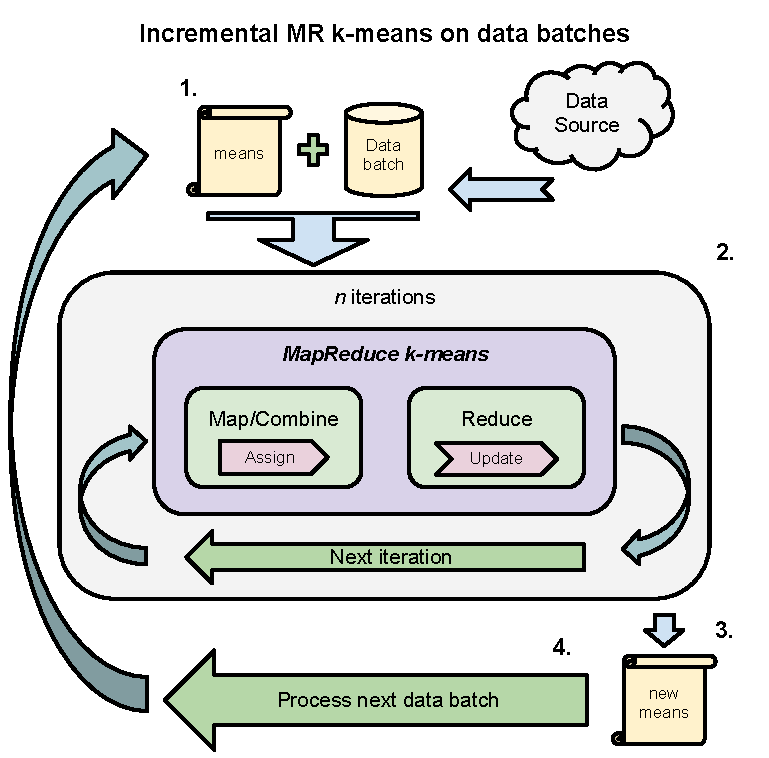
\includegraphics[width=1.0\textwidth]{Figures/IncrementalMRKmeansExecutionProcess.pdf}
\caption{The incremental MR k-means execution flow.}
\label{fig:mrkmeansprocess}
\end{figure}


\section{Development Environment and Tools}
The MapReduce k-means algorithm was implemented using a MR development framework called \textit{mrjob}~\footnote{http://pythonhosted.org/mrjob/}. Mrjob is a open-source Python framework actively maintained by Yelp~\footnote{http://opensource.yelp.com/}, that allows MapReduce jobs to be written in Python 2.5+ and executed on several platforms. Using mrjob allows for rapid implementation of MapReduce jobs by running them locally for development purposes and easily run them on your own Hadoop cluster or even easier using the Amazon Elastic MapReduce (Amazon EMR)\footnote{http://aws.amazon.com/elasticmapreduce/}. Amazon EMR is a web service that allows developers to buy time on a Hadoop cluster to process large-scale data easily and cost-effectively. Amazon EMR web service was used in the scalability and the nearest centroid experiments.

The Python programming language was chosen for this study because GameAnalytics (GA) also uses Python and mrjob to implement their MapReduce jobs. Allowing GA easily to use and build further on the implementation from this study. In this thesis, the NumPy/SciPy Python library that enables vectorisation approaches and array/matrix data structures for easier and more efficient data vector manipulations. The implementation of algorithms and running experiments were executed on a Linux operating system, recommended by GA instead of using a Windows OS, because of Python libraries compatibility and mrjob.

\newpage
\section{Experiments Set-up}
\label{sec:experimentsetup}
Several experiments were conducted to evaluate the MapReduce k-means algorithm, the experiments were:
\begin{enumerate}
	\item \textbf{Cluster Quality - Real Dataset}: Test the cluster quality and error stability when clustering incrementally multiple data batches of real game data.
	\item \textbf{Cluster Quality - Generated dataset}: Same as the first experiment, but using a generated multiple data batches with three normal distributions were the means are moving and changing slowly between batches.
	\item \textbf{General Player Behaviour}: Find and interpret the general player behaviour in the real game data, after incrementally clustering multiple data batches with MR K-means.
	\item \textbf{Scalability}: Measure the \textit{horizontal} (scale-out), \textit{vertical} (scale-up) and scaling both computing power and data size. Clustering a single set of generated dataset of different sizes and on different combinations of computers and processors. All measures are run using the Amazon EMR web service.
	\item \textbf{MR K-means Combiner vs. non-Combiner}: Compare the running time when the Combiner function is not implemented in the MapReduce execution flow.
	\item \textbf{Nearest Centroid Computation Methods}: Compare three different nearest centroid computation methods using Amazon EMR.
\end{enumerate}


\subsection{Experiment: Cluster Quality - Real Dataset}
\label{sec:experimentrealdata}
For this experiment the cluster quality or Sum of Squared Error (SSE) between multiple data batches was measured and how stable the error was. As described in Section~\ref{preprocessing} the user telemetry dataset needed to be preprocessed and split into ten data batches, where the data was timely ordered after the \textit{event} timestamp. Ten parts sounded a reasonable number and was therefor used for this experiment, leaving $\approx 510.000$ events for each part. For each part events were aggregated or counted to construct the game metric datasets used as input to the algorithm, each containing $\approx 13.500$ records of unique players, see Section~\ref{gamemetric} for the game metric feature selection. 

Having these ten timely ordered datasets we are simulating the environment were new chunks of game data arrive each day from a game, like in GameAnalytics. In Figure~\ref{fig:realdatasubfigures} we can see an example how four of the ten data batches look like in $2$-d, after running the normal iterative k-means implementation in the Python scientific library SciPy.

The MR k-means algorithm in Section~\ref{sec:MapCombineReduceVersion} was executed locally instead of using Amazon EMR. Using the Python mrjob MR development framework the MapReduce environment and its execution flow is simulated locally instead running it on e.g. Hadoop instances in Amazon EMR, this was done to save time and should not affect the results.

\begin{figure}[ht!]
        \begin{center}
        \subfigure{%
            \label{fig:first}
            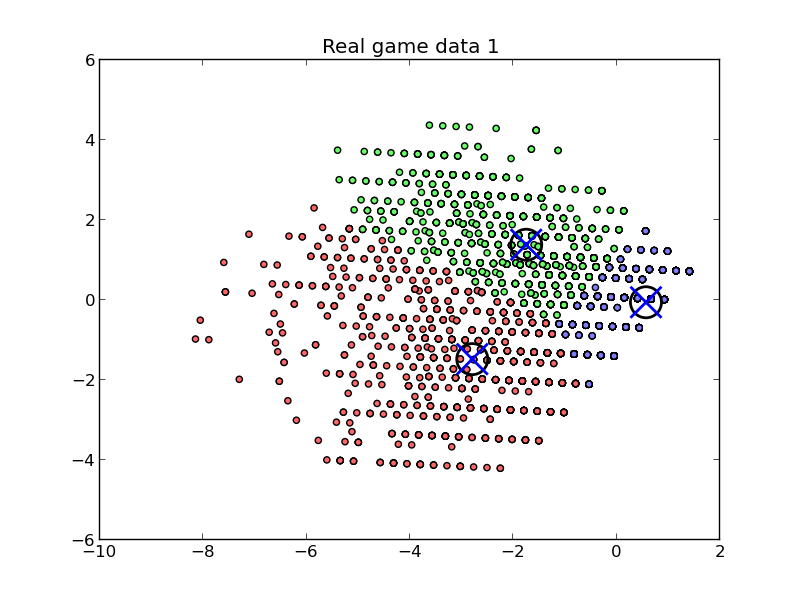
\includegraphics[width=0.5\linewidth]{Figures/realdata/0_realdata_2d.png}
        }%
        \subfigure{%
           \label{fig:second}
           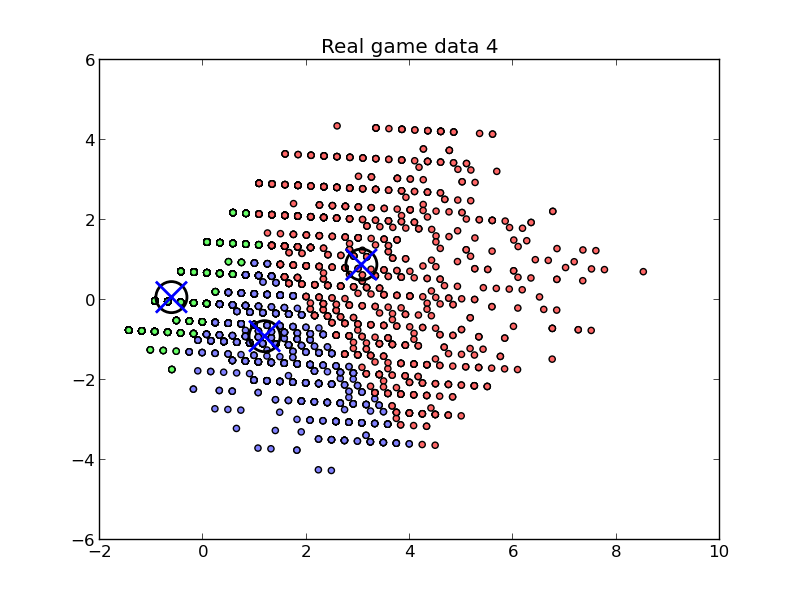
\includegraphics[width=0.5\textwidth]{Figures/realdata/3_realdata_2d.png}
        } %  ------- End of the first row ----------------------%
        \subfigure{%
            \label{fig:third}
            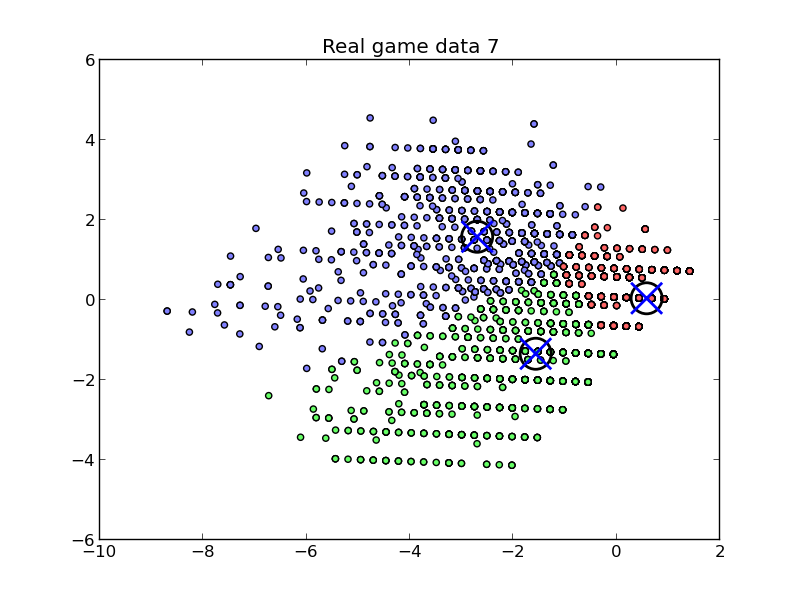
\includegraphics[width=0.5\textwidth]{Figures/realdata/6_realdata_2d.png}
        }%
        \subfigure{%
            \label{fig:fourth}
            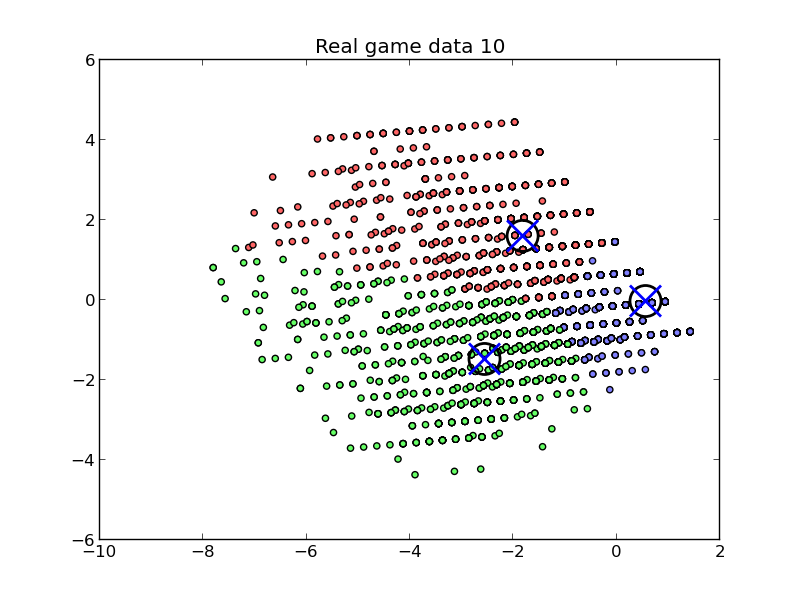
\includegraphics[width=0.5\textwidth]{Figures/realdata/9_realdata_2d.png}
        }%
        \end{center}
    \caption{In this figure we can see four of the ten data batches that were used in the experiment when measuring the cluster quality for multiple real game datasets. The data batches are $3$-dimensional and were projected to $2$-dimensional for better visualization, using Principal component analysis.}
   \label{fig:realdatasubfigures}
\end{figure}

Three different methods were compared to measure the cluster quality for each data batch over multiple batches. These methods test different number of iterations that we run the MR k-means algorithm  on each data batch, the methods are following:
\begin{itemize}
\item $1$-iteration
\item $2$-iterations
\item $5$-iterations
\end{itemize}

Ten experiments were performed each with different random initial centroids selected from the first data batch. For all the methods we start with the same initial centroids and parameters; number of centroids $k=3$ and the minimum change in centroids, $threshold\_delta = 0.01$, if below threshold the iteration loop exits before finishing the $n$ iterations. Each experiment executes the following steps:
\begin{enumerate}
	\item Continue until no more data batches.
	\item Select the next data batch.
	\item Select intermediate centroids \textit{(If the first batch, then use the initial centroids)}.
	\item Execute the MapReduce k-means program with a $n$-iteration method of choice.
	\item Calculate the SSE.
	\item Store the intermediate centroids received after $n$-iterations.
\end{enumerate}

The MapReduce k-means program (see Algorithm~\ref{alg:mrkmeansprogram}) controls the iterations of the MR k-means algorithm (see Section~\ref{sec:MapCombineReduceVersion}).

\subsection{Experiment: Cluster Quality - Generated Dataset}
Same measurements, setups and execution flow were performed for this experiment like the experiment in Section~\ref{sec:experimentrealdata}, except generated data batches were used instead of the real game data set. The generated dataset was also split up into ten data batches, each containing $3.000$ $2$-dimensional records. 

The idea with this experiment is that the fictive data was generated with three normal distributions where they move between data batches. In the first data batch all three means are very close together. In the next data batches the means move little bit further away from each other and also the population in two of the clusters changes over time, where the furthest one (up-right) loses data points while the lower to the left gains those points, this was tried to simulate that less extremes are found in reality than the majority of the population. We can see in Figure~\ref{fig:generateddatasubfigures} how the means move between data batches.

\begin{figure}[ht!]
        \begin{center}
        \subfigure[Three means start close together]{%
            \label{fig:first}
            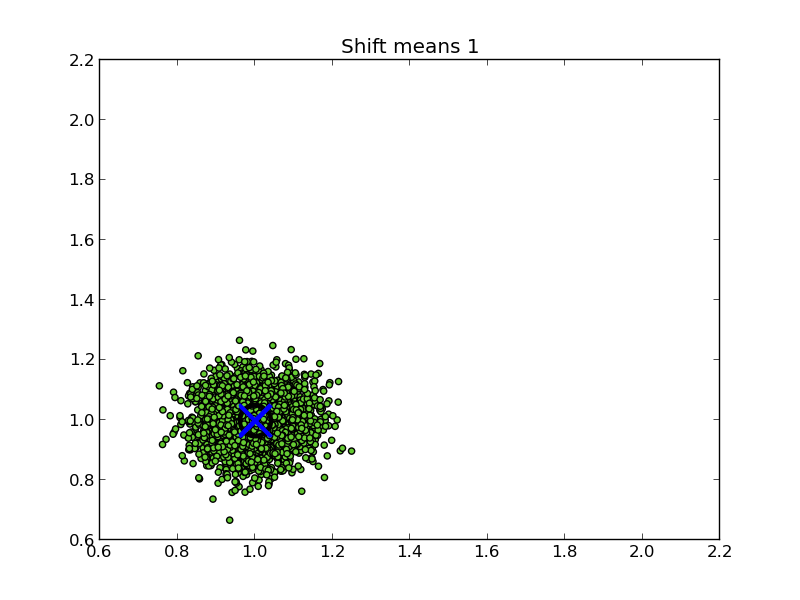
\includegraphics[width=0.5\linewidth]{Figures/gmeans/0_genshiftmeans.png}
        }%
        \subfigure[The means are moving a little bit]{%
           \label{fig:second}
           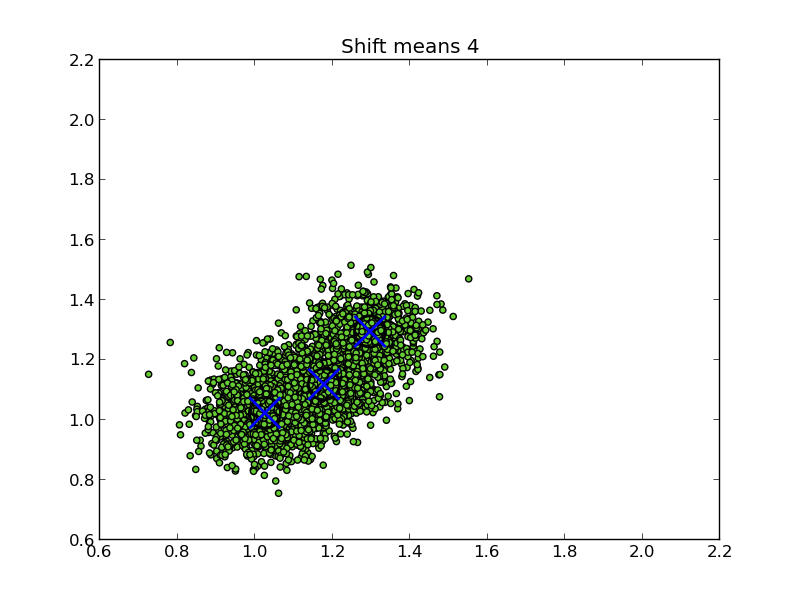
\includegraphics[width=0.5\textwidth]{Figures/gmeans/3_genshiftmeans.png}
        } %  ------- End of the first row ----------------------%
        \subfigure[Three distributions can now be spotted]{%
            \label{fig:third}
            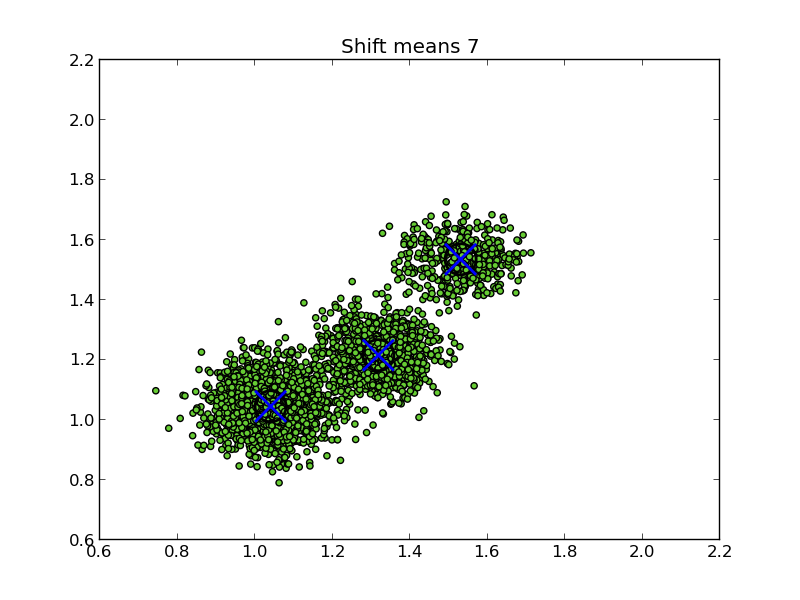
\includegraphics[width=0.5\textwidth]{Figures/gmeans/6_genshiftmeans.png}
        }%
        \subfigure[One mean has moved away from the crowd and with fewer points]{%
            \label{fig:fourth}
            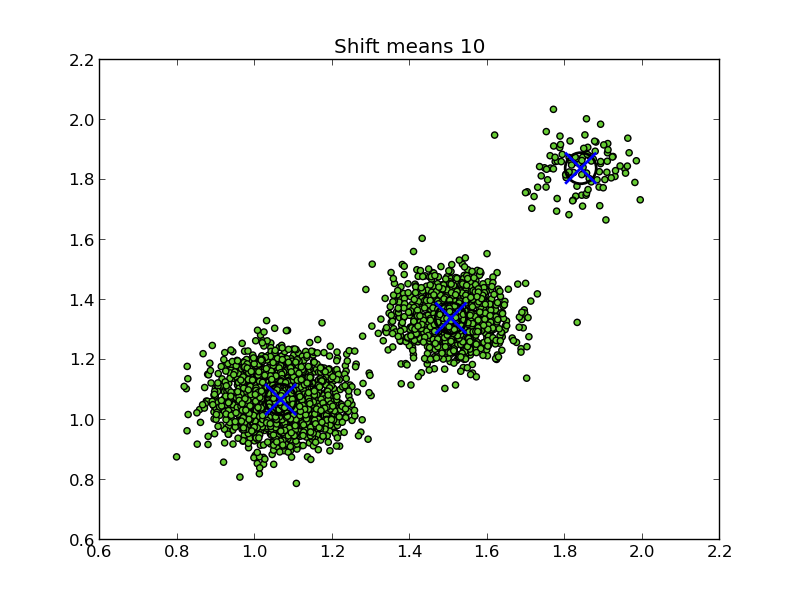
\includegraphics[width=0.5\textwidth]{Figures/gmeans/9_genshiftmeans.png}
        }%
        \end{center}
    \caption{In this figure we can see four of the ten datasets that were used in the experiment when measuring the cluster quality for multiple generated datasets.}
   \label{fig:generateddatasubfigures}
\end{figure}

As mentioned the experiment was executed with same setup, parameters and the same methods were compared as described in the other cluster quality experiment for the real data in Section~\ref{sec:experimentrealdata}.

\subsection{Experiment: General Player Behaviour}
\label{sec:experiment_gpb}
In this experiment three general player behaviour groups were extracted and interpreted from the the real game dataset in Section~\ref{sec:realdataset}, contributed by GameAnalytics. 

The results from the cluster quality experiment in Section~\ref{sec:experimentrealdata} were used and analyzed for this experiment. The $n$-iteration method that gave the most stable SSE error results was selected, where multiple data batches were clustered incrementally. The final means that had the lowest SSE after the last data batch was used to represent the general player behaviour for the data batches. 

The means uses were z-score values (Standardize values, see preprocessing in Section~\ref{preprocessing}) and were converted to the original range of values, by transforming z-score formula to find the original value as follows

\begin{center}
$x = (z * \sigma) + \mu$ 
\end{center}

where $x$ is the original value in the original numeric range and $z$ is the z-score value. The standard deviation $\sigma$ and average $\mu$ were calculated from the original range for that data batch.

\subsection{Experiment: Scalability}
\label{sec:experimentscalability}
High scalability of the MR k-means algorithm is very important when the datasets increases in sizes. The MapReduce framework offers high scalability out of the box in its execution flow, favoring scale-out instead of scale-up with the idea of distributing a large-scale work to a large number of commodity low-end servers instead of a few expensive high-end servers. Multiple computers work on each piece of the data in parallel and all the intermediate results in a fault tolerance are combined in the end. An algorithm must also be efficient and well written with parallel processing in mind to take a full advantage of the MapReduce framework.

All experiments were run using The Amazon Elastic MapReduce (Amazon EMR) Web Service~\footnote{http://aws.amazon.com/elasticmapreduce/}. Offering vast possibilities to easily configure and run various Hadoop clusters instances on the Amazon Elastic Compute Cloud (Amazon EC2) on-demand. 

All datasets were generated with three normal distributions in $3$-dimension. The data points were shuffled (using NumPy shuffle) such that they represent a random order internally, avoiding bias when the MapReduce framework is splitting up the data to be distributed. All datasets were uploaded to the Amazon Simple Storage (Amazon S3) providing fast and safe data transfer to and from the Amazon EC2 Hadoop instances.

The MR k-means algorithm (in Section~\ref{sec:MapCombineReduceVersion}) was measured using the $1$-iteration method, that is the algorithm runs only one iteration on the dataset. The running time of the algorithm was taken from the MapReduce system log file where it states when the job starts running and completes, excluding e.g. the extra overhead when starting the MR job directly from the MR k-means program, see Section~\ref{sec:mrkmeansprogram}.

The scalability of the MR k-means algorithm was measured by conducting the following experiments:
\begin{itemize}
	\item Horizontal scaling (Scale-out): Number of computer nodes are doubled, same dataset size.
	\begin{itemize}
		\item Dataset: 220 MB.
		\item EC2 Type: 5 Compute Unit (2 cores x 2.5 units), High-CPU Medium.
		\item Nodes setup: 2, 4, 6 and 8.
	\end{itemize}
	\item Vertical scaling (Scale-up): The computing power is doubled, same dataset size.
	\begin{itemize}
		\item Dataset: 220 MB.
		\item EC2 Type: 1 Compute Unit (1 core x 1 unit),  M1 Small.
		\item EC2 Type: 2 Compute Unit (1 core x 2 units), M1 Medium.
		\item EC2 Type: 4 Compute Unit (2 cores x 2 units), M1 Large.
		\item EC2 Type: 8 Compute Unit (4 cores x 2 units), M1 Extra Large.
		\item Nodes setup: 2
	\end{itemize}
	\item Scaling: The dataset is doubled in parallel when doubling the number of processor nodes.
	\begin{itemize}
		\item Dataset: 220 MB and 2 nodes.
		\item DataSet: 440 MB and 4 nodes.
		\item Dataset: 880 MB and 8 nodes.
		\item Dataset: 1.760 MB and 16 nodes.
		\item EC2 Type: 5 Compute Unit (2 cores x 2.5 units), High-CPU Medium.
	\end{itemize}
\end{itemize}

\subsection{Experiment: MR K-means Combiner vs. non-Combiner}
Compared the running time for the MR k-means algorithm with the Combiner function removed from the MR execution flow, see Section~\ref{sec:MapCombineReduceVersion} for the algorithm details.

The Amazon EMR web service was used for measuring the running time for the two algorithms. The cluster setup was the same for both algorithms when processing different sizes of datasets. The datasets are the same as explained in the experiment in Section~\ref{sec:experimentscalability}, also the running time was taken from the MapReduce system log inside Amazon EMR.

The experiment set-up:
\begin{itemize}
	\item Dataset: 220 MB, 440 MB, 880 MB and 1.760 MB.
	\item EC2 Type: 20 Compute Unit (8 cores x 2.5 units). High-CPU Extra Large.
	\item Nodes setup: 4
\end{itemize}


\subsection{Experiment: Nearest Centroid Computation Methods}
The three different methods of computing the nearest centroid, that is finding the centroid that has the minimum Euclidean distance between a data point in a dataset, were measured and compared. The most computation work in the MR k-means algorithms is finding the nearest centroid for each point that is being processed in the Mapper function. The implementation of the methods are explained in Section~\ref{sec:kmeansfinalversion} and \ref{sec:alternativenearestcentroid}. They are:

\begin{itemize}
\item Naive version: For loops, iterating over all features for all $k$ centroids calculating the squared error for each data point. 
\item Vectorisation - NumPy: Using a special NumPy $n$-dimensional array object, allowing efficient operations without use of for loops.
\item Distance matrix - SciPy: Loading all the data points into memory and find the distance matrix to find nearest centroids for all data points in a super fast way but with high memory cost.
\end{itemize}

Two experiments were conducted on Amazon EMR:
\begin{itemize}
	\item Dataset: 220MB.
	\item EC2 Type: 5 Compute Unit (2 cores x 2.5 units), High-CPU Medium.
	\item Nodes setup: 4, 6, 8, 10
\end{itemize}

The datasets are the same as explained in the experiment in Section~\ref{sec:experimentscalability}, also the running time was taken from the MapReduce system log inside Amazon EMR.

\subsection{About the experiments}
Here are some general notes when the experiments were conducted:

\begin{itemize}
\item It takes time to fire up a MR job on a new on-demand EC2 instance on Amazon EMR. The process of starting the instance, bootstrapping can take up to 5 minutes. To safe time a \textit{Job Flow} was created and used, to start an EC2 instance with out a MR job. After that it is possible to run jobs quickly by assigning them to a available job flow. (Useful when doing e.g. $n$-iterations of the MR k-means job)
\item The default EC2 instance type for the Master Controller node for all the experiments when running on Amazon EMR was: Compute Unit 1 (1 core x 1 unit), M1 Small.
\item Config file for mrjob: Needed to set the Hadoop version to $1.0.3$ for all instances to be able have the newest batches/updates, such as NumPy/SciPy scientific libraries.
\item The parameters for number of centroids $k=3$ and the $threshold\_delta = 0.01$ was kept from the start of the implementation and to the end of the experimentation process. The idea was to focus on few groups than too many and stop a k-means iteration process if the means moved less than $1\%$ between iterations. Tuning these parameters were not under a scope for this thesis.
\item The initial $k$ centroids for the MR k-means algorithm was always picked randomly from the dataset under test. When doing comparisons then the initial centroids were stored beforehand and tests under question would use the same centroids.
\end{itemize}























